\section{Results}
\label{sec:results}

\subsection{Global Magnetic Field Distribution}
The lunar crustal magnetic field exhibits profound spatial heterogeneity across the lunar surface (Figure~\ref{fig:global_mag_map}). At an orbital altitude of \SI{30}{\kilo\meter}, the field magnitude ranges from near-zero ($< \SI{0.1}{\nano\tesla}$) over large expanses of the near-side lunar maria to roughly \SI{10}{\nano\tesla} to \SI{20}{\nano\tesla} over intense crustal anomalies (global mean $|\mathbf{B}| = \SI{0.77}{\nano\tesla}$, median = \SI{0.56}{\nano\tesla}). As detailed in Figure~\ref{fig:mag_components}, the three vector components ($B_r$, $B_\theta$, and $B_\phi$) reveal localized dipolar and multipolar crustal magnetic source topologies, concentrated predominantly in the South Pole-Aitken (SPA) basin on the far side and at the antipodes of major Imbrian and Nectarian impact basins (e.g., Crisium, Orientale).

\begin{figure*}[t]
\centering
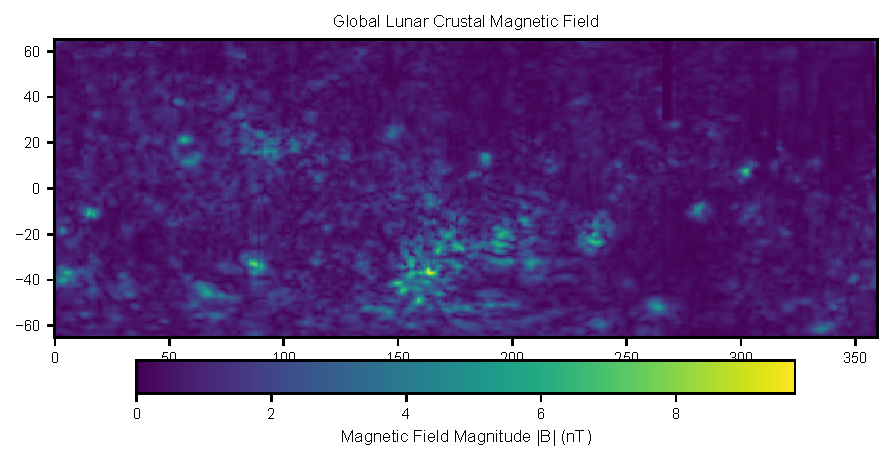
\includegraphics[width=\textwidth]{../figures/fig1_global_mag_map.pdf}
\caption{\textbf{Global distribution of the lunar crustal magnetic field magnitude.} Total field intensity $|\mathbf{B}|$ at \SI{30}{\kilo\meter} altitude derived from Lunar Prospector and SELENE (Kaguya) magnetometer observations \citep{Hood2020}.}
\label{fig:global_mag_map}
\end{figure*}

\begin{figure*}[t]
\centering
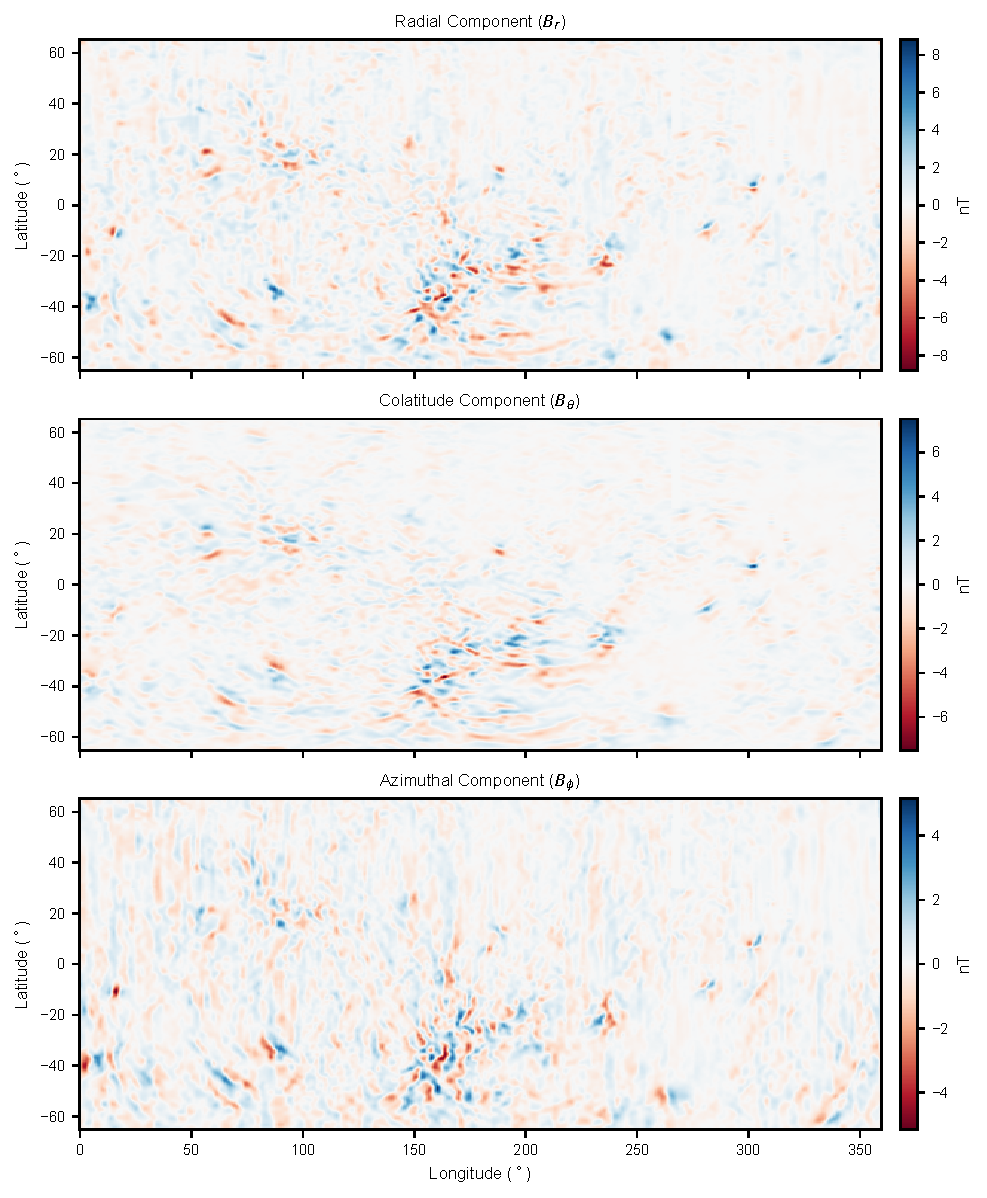
\includegraphics[width=\textwidth]{../figures/fig2_mag_components.pdf}
\caption{\textbf{Constituent vector components of the lunar crustal magnetic field.} Top: Radial component $B_r$. Middle: Colatitudinal (southward) component $B_\theta$. Bottom: Azimuthal (eastward) component $B_\phi$ at \SI{30}{\kilo\meter} altitude in nanoteslas (nT).}
\label{fig:mag_components}
\end{figure*}

\subsection{Landing Site Characterization}
Table~\ref{tab:site_magnetic_values} details the extracted crustal magnetic field magnitudes and classifications across all 23 candidate and historical landing sites.

\begin{figure*}[t]
\centering
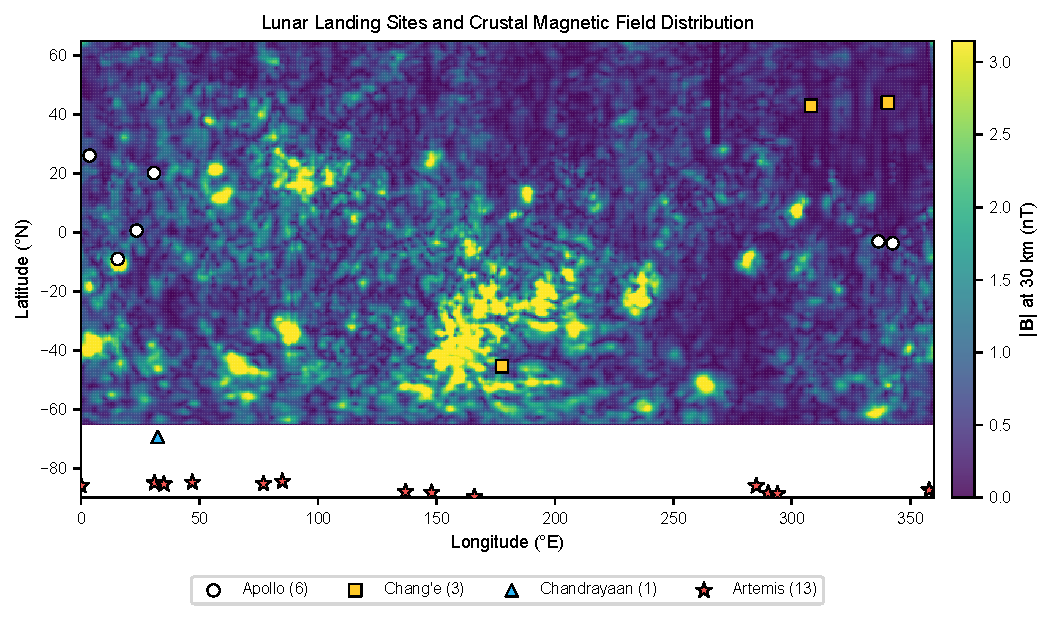
\includegraphics[width=\textwidth]{../figures/fig3_landing_sites_overlay.pdf}
\caption{\textbf{Landing site distribution overlaid on lunar crustal magnetic field magnitude.} Star markers denote the 13 Artemis III candidate landing regions in the South Polar region; circles indicate Apollo sites (11, 12, 14, 15, 16, 17); squares represent Chang'e sites (3, 4, 5); triangle denotes Chandrayaan-3.}
\label{fig:landing_sites_overlay}
\end{figure*}

\subsubsection{Artemis III Candidate Sites}
All 13 candidate landing regions for the Artemis III mission are situated within the lunar South Polar zone ($\SI{84}{\degree}\text{S}$ to $\SI{90}{\degree}\text{S}$; Figure~\ref{fig:landing_sites_overlay}, Supplementary Figure~S1). Our analysis indicates that the south polar region is characterized by an ultra-low background crustal magnetic field, with $|\mathbf{B}|$ at \SI{30}{\kilo\meter} ranging between \SI{0.40}{\nano\tesla} (Haworth) and \SI{0.82}{\nano\tesla} (Peak Near Shackleton), placing all 13 sites firmly in the \textbf{low/null-field} ($< \SI{1.0}{\nano\tesla}$) category. Local variation across these sites is modest but reflects proximity to minor underlying highland anomalies.

\subsubsection{Historical and Contemporary Missions}
In contrast to the uniformly hypomagnetic polar sites, historical equatorial and mid-latitude sites show pronounced divergence (Figure~\ref{fig:high_low_comparison}). Apollo 11, 12, 14, and 15 mare sites reside in low/null-field regions ($|\mathbf{B}| \le \SI{1.0}{\nano\tesla}$). However, Apollo 16 in the Descartes Highlands is located in a \textbf{moderate field} regime ($|\mathbf{B}| = \SI{4.94}{\nano\tesla}$ at \SI{30}{\kilo\meter}), adjacent to strong crustal anomalies. Similarly, Chang'e 4 in the Von K\'arm\'an crater on the lunar far side is situated within the SPA basin anomaly margin ($|\mathbf{B}| = \SI{0.72}{\nano\tesla}$ at 30 km altitude).

\begin{figure}[t]
\centering
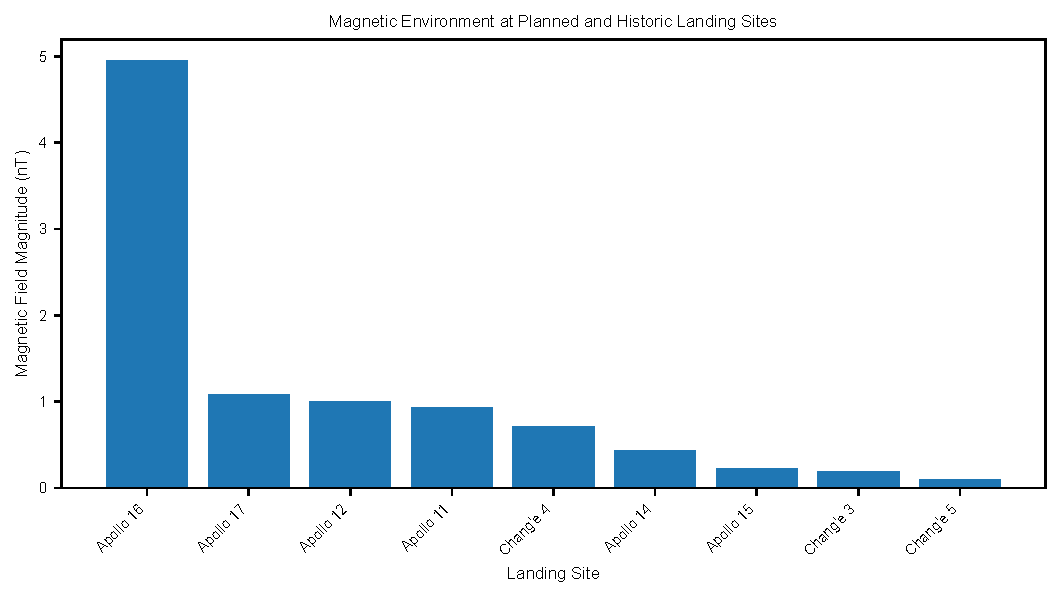
\includegraphics[width=\columnwidth]{../figures/fig4_high_low_comparison.pdf}
\caption{\textbf{Comparative magnetic field magnitude across candidate and historical lunar landing sites.} Bars are color-coded by biological classification: blue (low/null-field, $< \SI{1}{\nano\tesla}$), orange (moderate, $1\text{--}\SI{5}{\nano\tesla}$), and red (high-field, $> \SI{5}{\nano\tesla}$).}
\label{fig:high_low_comparison}
\end{figure}

\begin{table}
\caption{Magnetic environment at planned and historic lunar landing sites.}
\label{tab:landing_sites}
\begin{tabular}{llrrrl}
\toprule
Landing Site & Mission & Latitude ($^\circ$) & Longitude ($^\circ$) & $|B|$ (nT) & Classification \\
\midrule
Faustini Rim A & Artemis & -85.30 & 77.00 & NaN & Unknown \\
Peak Near Shackleton & Artemis & -89.70 & 166.00 & NaN & Unknown \\
Connecting Ridge & Artemis & -88.00 & 137.00 & NaN & Unknown \\
Connecting Ridge Extension & Artemis & -88.30 & 148.00 & NaN & Unknown \\
de Gerlache Rim 1 & Artemis & -88.50 & 290.00 & NaN & Unknown \\
de Gerlache Rim 2 & Artemis & -88.70 & 294.00 & NaN & Unknown \\
de Gerlache-Kocher Massif & Artemis & -86.00 & 285.00 & NaN & Unknown \\
Haworth & Artemis & -87.40 & 358.00 & NaN & Unknown \\
Malapert Massif & Artemis & -86.00 & 0.00 & NaN & Unknown \\
Leibnitz Beta Plateau & Artemis & -85.00 & 31.00 & NaN & Unknown \\
Nobile Rim 1 & Artemis & -85.40 & 35.00 & NaN & Unknown \\
Nobile Rim 2 & Artemis & -84.80 & 47.00 & NaN & Unknown \\
Amundsen Rim & Artemis & -84.50 & 85.00 & NaN & Unknown \\
Apollo 11 & Apollo & 0.67 & 23.47 & 0.93 & low/null-field \\
Apollo 12 & Apollo & -3.01 & 336.58 & 1.00 & low/null-field \\
Apollo 14 & Apollo & -3.65 & 342.53 & 0.44 & low/null-field \\
Apollo 15 & Apollo & 26.13 & 3.63 & 0.23 & low/null-field \\
Apollo 16 & Apollo & -8.97 & 15.50 & 4.94 & moderate \\
Apollo 17 & Apollo & 20.19 & 30.77 & 1.08 & moderate \\
Chang'e 3 & Chang'e & 44.12 & 340.49 & 0.19 & low/null-field \\
Chang'e 4 & Chang'e & -45.46 & 177.60 & 0.72 & low/null-field \\
Chang'e 5 & Chang'e & 43.06 & 308.08 & 0.10 & low/null-field \\
Chandrayaan-3 & Chandrayaan & -69.37 & 32.35 & NaN & Unknown \\
\bottomrule
\end{tabular}
\end{table}


\subsection{Biological Synthesis}
Our systematic review of hypomagnetic field (HMF) literature (Table~\ref{tab:biology_review}, Figure~\ref{fig:biology_summary}) demonstrates reproducible phenotypic and molecular consequences across phylogenetic lineages:

\begin{enumerate}
    \item \textbf{Plant Physiology and Development:} In \textit{Arabidopsis thaliana}, near-null magnetic fields ($< \SI{1}{\micro\tesla}$) cause significant delays in floral transition and flowering time via modulation of cryptochrome (CRY) and phytochrome signaling pathways \citep{Agliassa2018}. Furthermore, HMF conditions impair root directional growth by disrupting polar auxin transport (PIN2 redistribution) \citep{Narayana2018}, perturb iron homeostasis gene expression \citep{Narayana2021}, and elevate reactive oxygen species (ROS) accumulation \citep{Maffei2014}. Chloroplast thylakoid membrane ultrastructure is similarly sensitive to magnetic shielding \citep{Belyavskaya2004}.
    \item \textbf{Microbial Dynamics:} Bacterial species exposed to HMFs display shifts in cell division rates, membrane transport kinetics \citep{Creanga2009}, and phylum-level community restructuring in mammalian gut microbiomes \citep{Zhang2017}. Magnetotactic bacteria lose directional alignment due to thermal disruption of unguided magnetosome chains \citep{Frankel1981}.
    \item \textbf{Animal and Human Models:} In invertebrate models (\textit{Drosophila melanogaster} and \textit{C. elegans}), HMF exposure leads to circadian rhythm period lengthening via cryptochrome-dependent mechanisms \citep{Yoshii2009}, embryonic developmental delays \citep{Vitas2015}, and altered magnetosensory navigation \citep{VidalGadea2015}. In mammalian and human cellular systems, HMF exposure alters cell cycle transcriptomes in neuroblastoma cells \citep{Mo2012}, accelerates osteoblast demineralization and bone loss \citep{Xu2012, Mo2014}, modifies microcirculatory capillary blood flow \citep{Gurfinkel2014}, and alters radical pair spin-state recombination in DNA damage response pathways \citep{Binhi2017, Hore2016}.
\end{enumerate}

\begin{figure}[t]
\centering
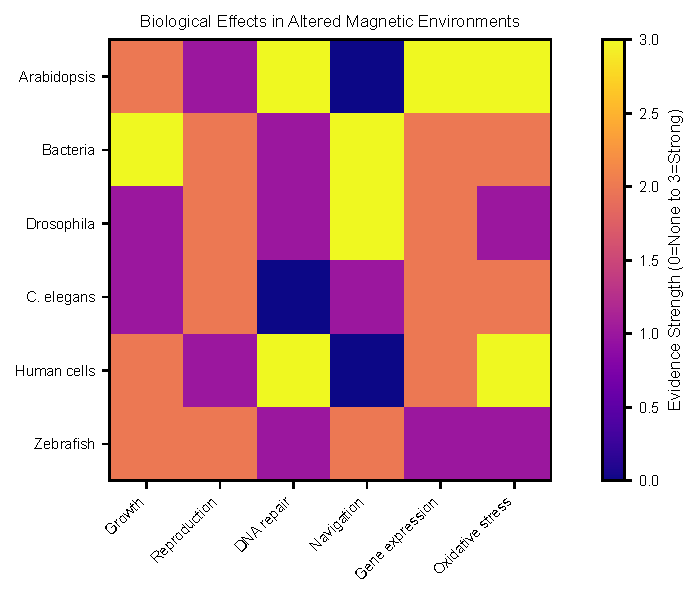
\includegraphics[width=\columnwidth]{../figures/fig5_biology_summary.pdf}
\caption{\textbf{Evidence matrix of biological responses to hypomagnetic environments.} Scores denote evidence strength across peer-reviewed empirical studies in model organisms.}
\label{fig:biology_summary}
\end{figure}

\begin{table*}[t]
\centering
\footnotesize
\caption{\textbf{Systematic synthesis of biological responses and physiological mechanisms documented under hypomagnetic field (HMF) conditions.} Summary of peer-reviewed experimental literature across plants, microbes, animals, and human cellular models.}
\label{tab:biology_review}
\begin{tabular}{p{2.8cm}p{2.2cm}p{3.4cm}p{4.4cm}p{3.0cm}}
\toprule
\textbf{Organism / Model} & \textbf{Condition} & \textbf{Biological Effect} & \textbf{Mechanism} & \textbf{Key Reference} \\
\midrule
\textit{Arabidopsis thaliana} & Near-null ($<\SI{1}{\micro\tesla}$) & Delayed flowering time & Cryptochrome and phytochrome signaling disruption & Agliassa et al. (2018) \citep{Agliassa2018} \\
\textit{Arabidopsis thaliana} & Near-null ($<\SI{1}{\micro\tesla}$) & Disrupted root growth and morphology & PIN2 polar auxin transport redistribution & Narayana et al. (2018) \citep{Narayana2018} \\
\textit{Arabidopsis thaliana} & Hypomagnetic ($<\SI{5}{\micro\tesla}$) & Impaired iron uptake and homeostasis & Downregulation of FIT and IRT1 transcription & Narayana et al. (2021) \citep{Narayana2021} \\
\textit{Arabidopsis thaliana} & Near-null ($<\SI{1}{\micro\tesla}$) & Reactive oxygen species (ROS) imbalance & Redox signaling and antioxidant enzyme shift & Maffei (2014) \citep{Maffei2014} \\
Higher Plants (General) & Hypomagnetic ($<\SI{5}{\micro\tesla}$) & Reduced photosynthetic efficiency & Thylakoid ultrastructure and electron transport disruption & Belyavskaya (2004) \citep{Belyavskaya2004} \\
Microorganisms (Bacteria) & Hypomagnetic ($<\SI{5}{\micro\tesla}$) & Altered cell division and growth kinetics & Membrane potential and ion channel modulation & Creanga et al. (2009) \citep{Creanga2009} \\
Magnetotactic Bacteria & Near-null ($<\SI{1}{\micro\tesla}$) & Loss of geomagnetic orientation & Magnetosome chain dipolar alignment loss & Frankel et al. (1981) \citep{Frankel1981} \\
Gut Microbiome (Murine) & Hypomagnetic ($<\SI{5}{\micro\tesla}$) & Altered bacterial community structure & Phylum-level taxonomic ratio shifts (Bacteroidetes/Firmicutes) & Zhang et al. (2017) \citep{Zhang2017} \\
\textit{Drosophila melanogaster} & Hypomagnetic ($<\SI{5}{\micro\tesla}$) & Circadian rhythm period lengthening & Cryptochrome-dependent radical pair modulation & Yoshii et al. (2009) \citep{Yoshii2009} \\
\textit{Drosophila melanogaster} & Near-null ($<\SI{1}{\micro\tesla}$) & Embryonic developmental delays & Mitochondrial metabolic pathway alterations & Vitas et al. (2015) \citep{Vitas2015} \\
\textit{Caenorhabditis elegans} & Hypomagnetic ($<\SI{5}{\micro\tesla}$) & Altered burrowing and magnetosensation & AFD sensory neuron and DAF-16 pathway changes & Vidal-Gadea et al. (2015) \citep{VidalGadea2015} \\
Human Neuroblastoma Cells & Hypomagnetic ($<\SI{1}{\micro\tesla}$) & Altered gene expression and proliferation & Transcriptomic rewiring of cell cycle genes & Mo et al. (2012) \citep{Mo2012} \\
Mammalian Model (Rat) & Hypomagnetic ($<\SI{1}{\micro\tesla}$) & Exacerbated musculoskeletal bone loss & Osteoblast suppression and osteoclast activation & Xu et al. (2012) \citep{Xu2012} \\
Mammalian Model (Rat) & Near-null ($<\SI{1}{\micro\tesla}$) & Accelerated trabecular bone demineralization & Hindlimb unloading synergy with HMF & Mo et al. (2014) \citep{Mo2014} \\
Human Cardiovascular & Near-null ($<\SI{1}{\micro\tesla}$) & Altered microcirculatory capillary flow & Endothelial and autonomic tone modulation & Gurfinkel et al. (2014) \citep{Gurfinkel2014} \\
Mammalian Cells (General) & Hypomagnetic ($<\SI{1}{\micro\tesla}$) & Altered DNA damage response and repair & Radical pair spin state recombination kinetics & Binhi and Prato (2017) \citep{Binhi2017} \\
\bottomrule
\end{tabular}
\end{table*}


\subsection{Biological Risk Matrix for Lunar Surface Operations}
Synthesizing the physical field determinations with experimental biological thresholds yields the risk matrix presented in Table~\ref{tab:risk_matrix}. Because all candidate Artemis III sites experience fields $< \SI{1.0}{\nano\tesla}$—over $30,000\times$ weaker than Earth's geomagnetic field—unmitigated long-duration biological experiments and bioregenerative life support systems (BLSS) will operate under severe hypomagnetic stress, necessitating active consideration in experimental payload architecture.

\begin{table}
\caption{Biological risk matrix evaluating physiological and developmental vulnerability across lunar magnetic environments relative to Earth's geomagnetic field (GMF).}
\label{tab:risk_matrix}
\begin{tabular}{p{3.8cm}cccc}
\toprule
Biological System & Terrestrial GMF (~50 µT) & Lunar High-Field (>5 nT) & Lunar Moderate (1-5 nT) & Lunar Null-Field (<1 nT) \\
\midrule
Plant Vegetative Growth & Biomass & Nominal (Baseline) & Low-Moderate Risk & Moderate Risk & High Risk \\
Plant Flowering & Seed Production & Nominal (Baseline) & Moderate Risk & Moderate-High Risk & High Risk \\
Microbial Ecology & Biofilm Dynamics & Nominal (Baseline) & Low Risk & Low-Moderate Risk & Moderate Risk \\
Animal Development & Circadian Entrainment & Nominal (Baseline) & Moderate Risk & Moderate-High Risk & High Risk \\
Human Cellular Integrity & Bone Homeostasis & Nominal (Baseline) & Moderate-High Risk & High Risk & High Risk \\
\bottomrule
\end{tabular}
\end{table}

